\documentclass[12pt]{beamer}
\usepackage[utf8]{inputenc}
\usepackage[T1]{fontenc}
\usepackage{lmodern}
\usepackage[spanish]{babel}
\usetheme{Berlin}
\usepackage{graphicx}
\usepackage{ragged2e}
\begin{document}
	\author{Equipo 2}
	\title{Proyecto Final Métodos Numéricos}
	\subtitle{Crecimiento Bacteriano}
	%\logo{}
	\institute{Tecnológico de Monterrey}
	\date{26 de noviembre del 2021}
	\subject{Profesor Adolfo Centeno}
	\setbeamercovered{transparent}
	%\setbeamertemplate{navigation symbols}{}
		\begin{frame}[plain]
		\maketitle
	\end{frame} 
     \begin{frame}
    	\frametitle{Caso de Estudio: Ecuaciones Diferenciales}
    	\textbf{Realizamos 4 temas del curso de Ecuaciones diferenciales en la plataforma de Udacity}
        \includegraphics[width=10cm, height=8cm]{inv.png}
    \end{frame}
    \begin{frame}
    	\frametitle{Regla de Simpson}
    	\justify{Al aislar ciertos tipos de bacterias en medios con un grado de selectividad de bajo a medio, se recurren a herramientas técnicas, tal es el caso de pruebas metabólicas, reacciones de polimerasa en cadena, y resiembras en cultivos con mayor selectividad. Se hace uso del método simpson para calcular el área bajo la curva de P. fluorescens, para comparar dicho resultado con la bibliografía disponible y de esta manera obtener una “confirmación” más del organismo de interés a cultivar (Valclare, 2002).}
    \end{frame}
    \begin{frame}
    	\frametitle{Regla de Simpson}
    	\includegraphics[width=10cm, height=8cm]{simpson.png}
    \end{frame}
    \begin{frame}
    	\frametitle{Problema con Polinomio de Newton}
    	\justify{Se quiere determinar el crecimiento en incubadora de un organismo desconocido en orden para lograr determinar a qué género y a que especie pertenece así como para obtener más información, esto se logrará utilizando el método de polinomio de newton para descubrir cuántas unidades formadoras de colonias se generan en un plazo de 30 minutos. 
    		Matlab:}
    \end{frame}
    \begin{frame}
    	\frametitle{Polinomio de Newton}
    	\includegraphics[width=10cm, height=8cm]{newton.png}
    \end{frame}
    \begin{frame}
    	\frametitle{Regresión lineal}
    	\justify{El crecimiento bacteriano implica la división celular, llevando a un aumento exponencial del número de células iniciales de una población.\\
    			Excel:Para poder dar solución a una problemática de crecimiento bacteriano por este método, se graficara la absorbancia vs el tiempo que tarda en crecer una bacteria.}
    \end{frame}
    \begin{frame}
    	\frametitle{Regresión: Excel y Matlab}
    	\includegraphics[width=10cm, height=8cm]{regresion.png}
    \end{frame}
    \begin{frame}
    	\frametitle{Conclusiones}
    	\justify{Simpson:A partir del uso del método simpson podemos determinar el área bajo la curva de  la fase relevante del crecimiento bacteriano, tal y como se presenta con el uso de los dos softwares previamente mencionados. Como podemos ver por los resultados obtenidos se obtuvo un área bajo la curva que en sí concuerda con los resultados registrados de crecimiento de  P. fluorescens.\\Polinomio de Newton:En conclusión, los datos obtenidos nos permitieron definir a este organismo como el de una bacteria, de la misma manera nos arrojó el número de Unidades formadoras de colonias en 30 minutos, siendo este de 380 colonias.}
    \end{frame}
    \begin{frame}
    	\frametitle{Conclusiones}
    	\justify{Regresión lineal :Se logró determinar en qué tiempo se duplicarían las bacterias mediante un problema de regresión lineal, como se puede observar R elevado al 2 tiene un valor de 0.9518 por lo que se puede deducir que el modelo es bueno debido a qué este valor se considera bueno a partir de que sea mayor de 0.6\\Como podemos observar, así como en el archivo de Excel se puso obtener la misma gráfica en Matlab así como la ecuación lineal Y= 0.0037x-0.1347, obteniendo un coeficiente de correlación de 0.9756 lo cual es razonable ya que al sacar raíz cuadrad de R elevado 2 obtenida de excel da ese valor, se comprueba el modelo tanto como en un programa como en otro dándonos el mismo resultado. }
    \end{frame}
    \begin{frame}
    	\frametitle{Trello}
    		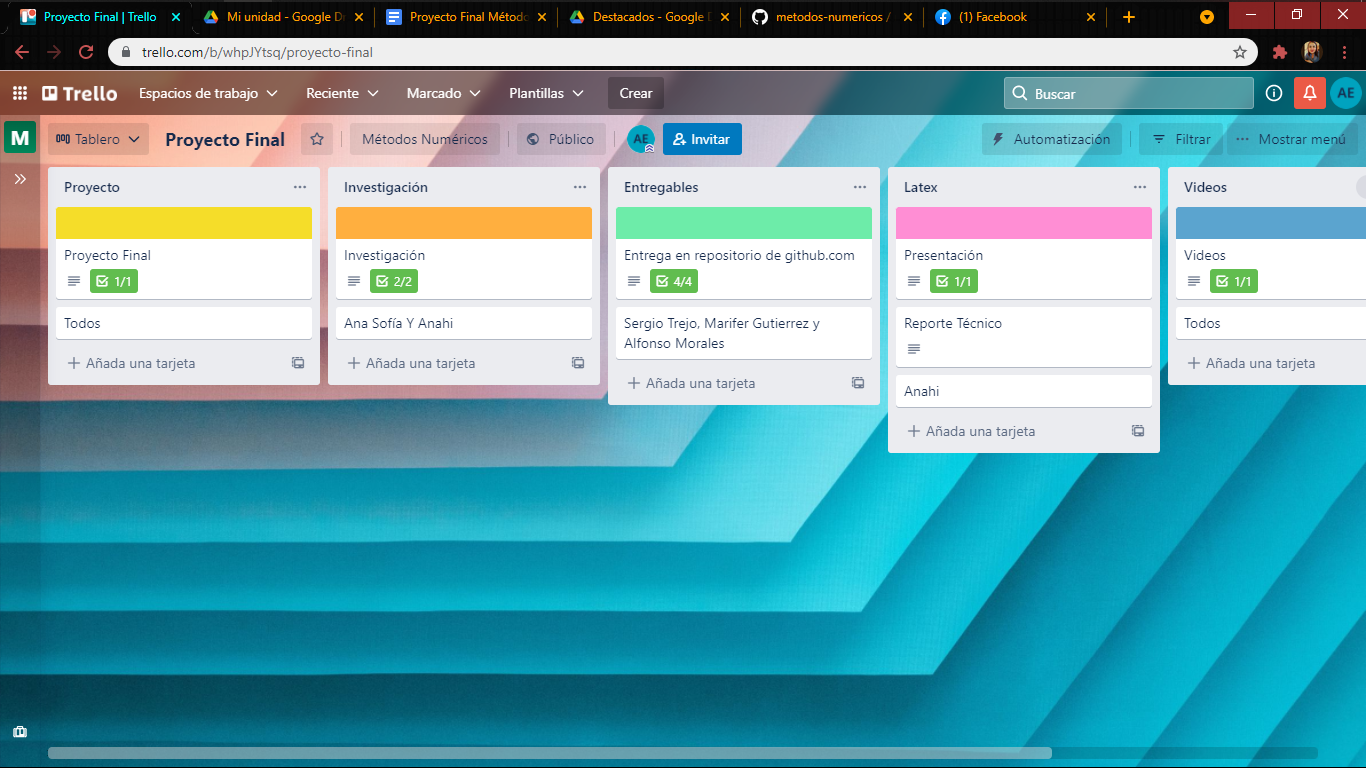
\includegraphics[width=10cm, height=8cm]{TrelloFinal.png}
    \end{frame}
    \begin{frame}
    	\frametitle{Repositorio}
    	\includegraphics[width=10cm, height=8cm]{repo.png}
    \end{frame}

\end{document} 
